\documentclass{article}
\usepackage[utf8]{inputenc}

\title{Generating artwork according to an emotional profile}
\author{Konrad Cybulski}
\date{March 2019}

\usepackage{natbib}
\usepackage{graphicx}

\begin{document}
	
\maketitle

\section{Introduction}

In the domain of creative artificial intelligence and evolutionary art, the desire exists for processes that produce imagery that is not only visually appealing, but images that exhibit abstract and emotive characteristics.
There exists extensive research on the production of realistic, and target label accurate images such as work by \citet{nguyen2015innovation} using quality-diverse (QD) algorithms in combination with deep neural networks (DNN), or \citet{bao2017cvae} that uses a variational generative adversarial network (GAN) architecture.
Recent work by \citet{tan2017artgan} has explored techniques for synthesizing artwork according to a target artist or genre through the use of a GAN architecture with highly accurate and creative results.

Little exploration however has been done on incorporating emotion into the process of art and image generation.
\citet{ali2017emotional} explored the idea of \textit{emotion transfer}, using techniques such as image emotion assignment, and color/style transfer with the aim of altering image composition to reach a target emotion.
Examples given use a target profile, with varying levels of emotions such as joy, anger, and fear, to alter the image's color composition.
The classification of an image's affective emotion, the emotion with which a viewer classifies the image, has been explored in various works \citep{machajdik2010affective, chen2015learning, kim2018building}.
\citet{kim2018building} produced a classifier for recognizing the emotion attributed to an image.
This was done through the application of a DNN to decompose an image to a two-dimensional feature vector (valence and arousal) representing the image's emotion mapped to a continuous plane (see Figure \ref{fig:valence-arousal}).

========================================

The work conducted by \citet{tan2017artgan} aimed to create a process by which artwork could be generated with more abstract characteristics. 
Through the use of a target artist or genre, and a respective discriminator assigned label, the generative network was able to produce images that were stylistically similar to the desired artist or genre.

There has been extensive research however into the synthesis of visually appealing and aesthetic images using evolutionary algorithms.
With human-guided evolution \citep{nevar} the process of fitness evaluation relies entirely on both subjective appeal, and unquantifiable metrics.
Quantifiably estimating the aesthetic appeal of an image has been studied by \citet{den2010comparing, den2010using, den2011evolving} with varying results.
A number of metrics such as image compression complexity, distribution of color gradients, fractal dimension, and contrast have shown to improve the quality of images generated through an unsupervised evolutionary process \citep{den2014investigating}.

========================================

Discuss the paper \citet{johnson2019understanding} which looks at the dissonance between aesthetic measures used in evolutionary art and the distributions of features ratings given by humans.

========================================

\section{Aims}

The aim of this research is to explore the synthesis of artwork with a target emotional profile.
Primarily leveraging work by \citet{tan2017artgan} and \citet{kim2018building} to produce a generative architecture whose output not only has desirable abstract characteristics, but shows emotive capabilities.
The proposed system would generate an image that satisfies a set of emotions provided.
This will investigate both the efficacy with which a generative system can create emotive images, as well as give insight into the properties attributed to various emotions portrayed in image form.

In order to test, and verify the output of such a system, generated images will be exhibited to explore their emotional effect on humans, and any dissonance between the intended, and resulting emotional profile.
This will further verify the accuracy with which an emotional profile can be synthesized into affective artwork with such an architecture.

\section{Background}

\subsection{Unsupervised image synthesis}

\begin{figure}[h!]
	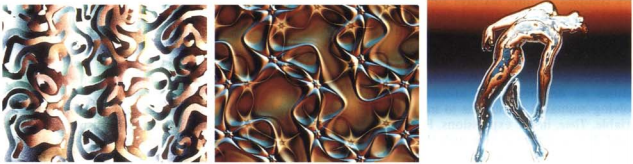
\includegraphics[width=\textwidth]{images/sims-interactive-image-generation.png}
	\caption{Images generated through the process of interactive evolution introduced by \citet{sims}}
	\label{fig:sims}
\end{figure}

The area of evolutionary art and image generation has been explored for many years.
Some of the first \textit{human-in-the-loop} systems such as \textit{NEvAr} \citep{nevar} produced greatly impressive images leveraging methods introduced and exemplified by \citet{sims} such as those shown in Figure \ref{fig:sims}.
\citet{sims} proposed using \textit{Lisp} expressions for genotype definitions, which accepted a coordinate (x, y) which could be evaluated into a grayscale or RGB value, thus producing images.
This genotype expression has been used in numerous further research into the process of both supervised and unsupervised image synthesis \citep{nevar, sims, den2011evolving, distributed-evolutionary-art, aesthetic-measures}.

\citet{sims} and \citet{nevar} were able to produce images with visually striking characteristics, despite the slow nature of the interactive process.
\citet{aesthetic-measures} investigated the use of measures of aesthetics for fitness evaluation in artificially evolving images.
This research primarily used the observation of \citet{ralph-bell-curve}, that the distribution of colour gradients in fine art tend towards normal.
While the images produced through this method did not meet the level of intricacy and detail as the results of \citet{sims} or \citet{nevar}, it represented a self-contained system able to generate appealing art without human interaction.

The introduction of the generative adversarial network architecture (GAN) by \citet{GAN} allowed the process of image generation to be completely unsupervised.
Common GAN application has involved the generation of realistic images, such as has been done by \citet{bao2017cvae}, where images have been synthesized to fine-detailed target labels such as bird species' and actors.
\citet{zhang2017stackgan} and \citet{reed2016generative} have recently explored text to image synthesis, in which detailed descriptions of birds and flowers have been converted into photo-realistic images using the GAN model.
\citet{tan2017artgan} has explored the generation of art according to target genre and artist.
Where throughout the training process,

\subsection{Deep neural networks for image classification and fitness evaluation}
Deep neural networks (DNN) have grown tremendously in popularity in the domain of image generation, and classification, and the accuracy with which they perform.

Research by \citet{burton1998genetic} showed that a genetic algorithm composing music benefited from fitness evaluation that relied on phenotype clustering, favoring those that showed diversity from existing clusters.

Recent work by \citet{nguyen2015deep} and \citet{nguyen2015innovation} has used pre-trained DNN image classifiers for fitness evaluation throughout the evolutionary process.
	
\subsection{Image emotion recognition}
	
\begin{figure}[h!]
	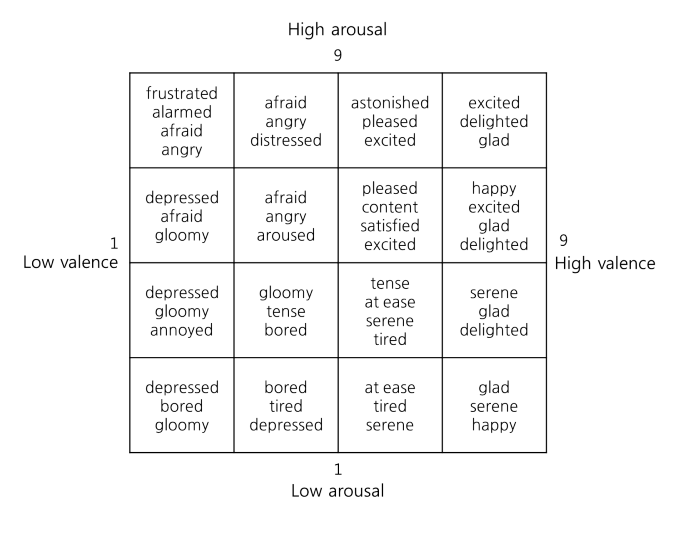
\includegraphics[width=0.75\textwidth]{images/valence-arousal-grid.png}
	\caption{Distribution of emotions associated with levels of valence and arousal determined by DNN classifier produced by \citet{kim2018building}}
	\label{fig:valence-arousal}
\end{figure}

\section{Methodology}


\section{Expected Outcomes \& Contributions}



\bibliographystyle{apalike}
\bibliography{references}

\end{document}
